\chapter{Einleitung}\label{ch:intro}






\section{Relevanz der Arbeit}

\textbf{Dies} ist unsere erste \textit{LaTeX-Vorlage.}


Wie in Abbildung 1.1 ersichtlich. 

\begin{figure}[h]
\centering
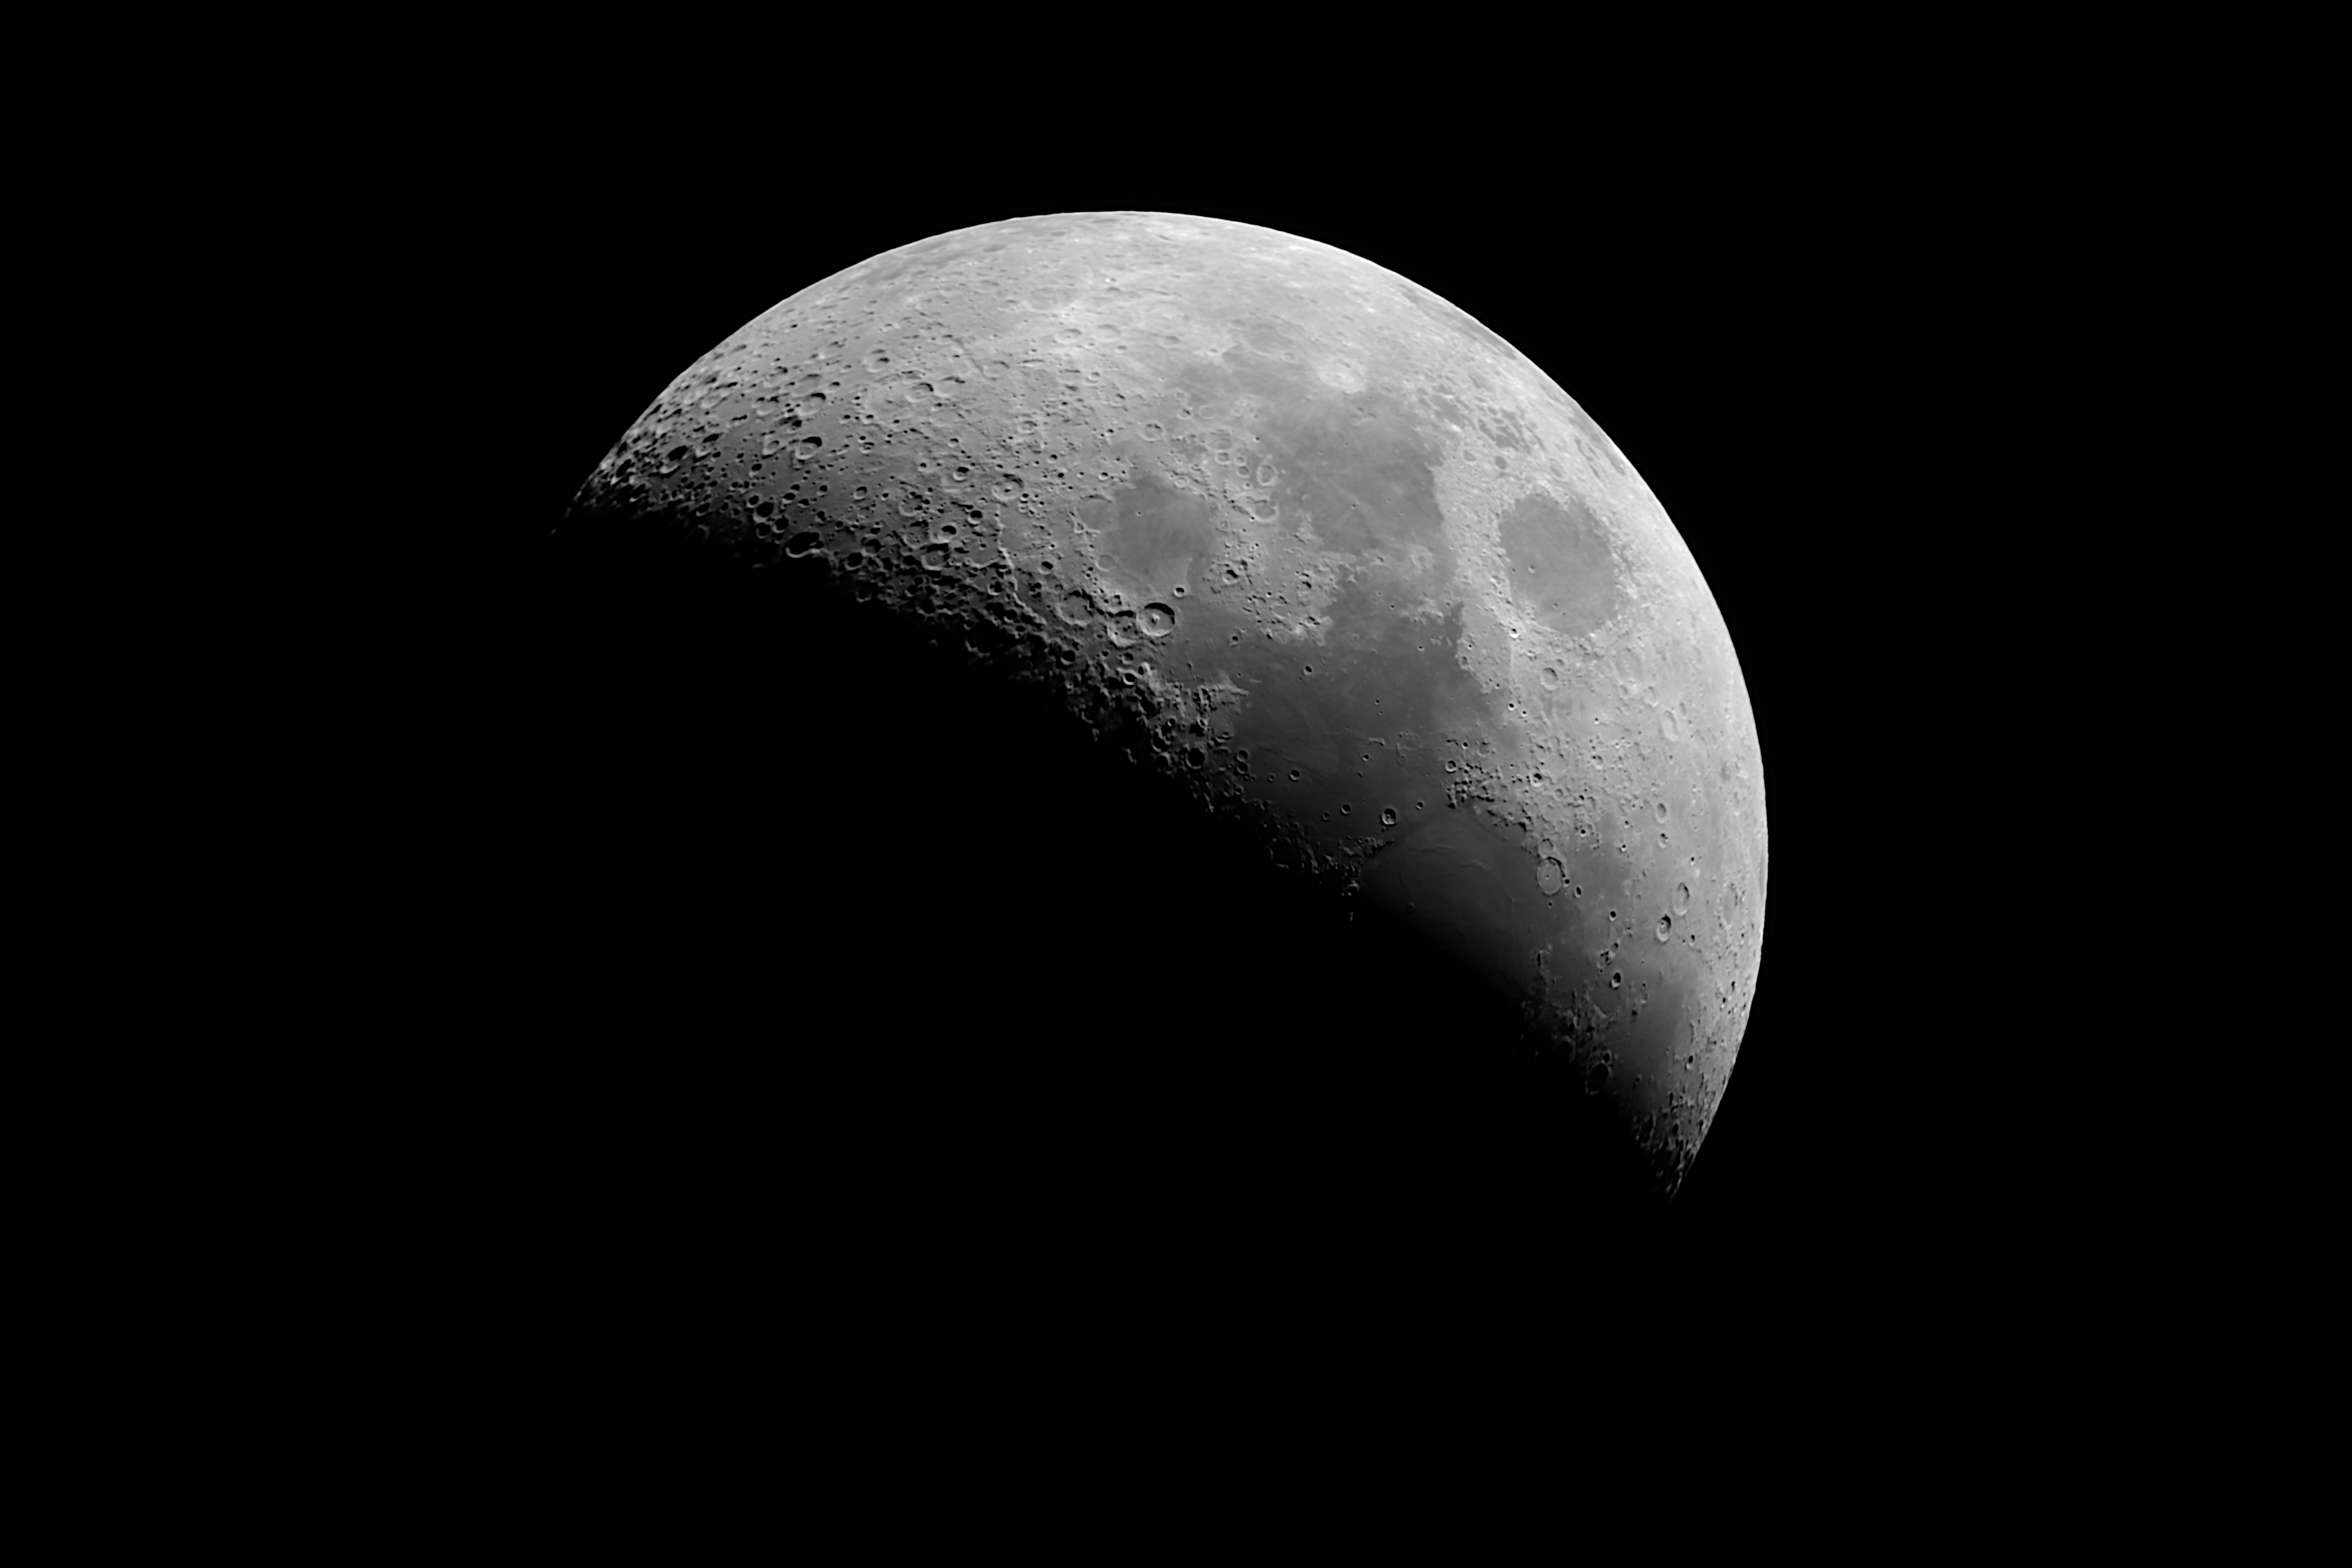
\includegraphics[width=8cm]{figures/Mond.jpg} %Bildbreite nach Belieben und ursprünglicher Bildgröße anpassen
\centering
\caption[Unser Mond]{Unser Mond (Quelle: Eigene Darstellung)}
\label{fig:Mond3}
\end{figure}



\begin{table}[htbp]
\centering
\caption{Unsere erste Tabelle}
\label{table:Tabelle1}
\begin{tabular}{r|c|l} %in der Spalte r:rechts, c: mittig oder l:links angeordnet
\hline %zwei Linien
Mond & Jupiter & Saturn\\
\hline\hline
… & …& … \\
\hline %eine Linie
… & … & …\\
\hline\hline
\end{tabular}
\end{table}


\begin{table}[htbp]
\caption{Konzeptmatrix}
\label{tab:Konzeptmatrix}
\centering
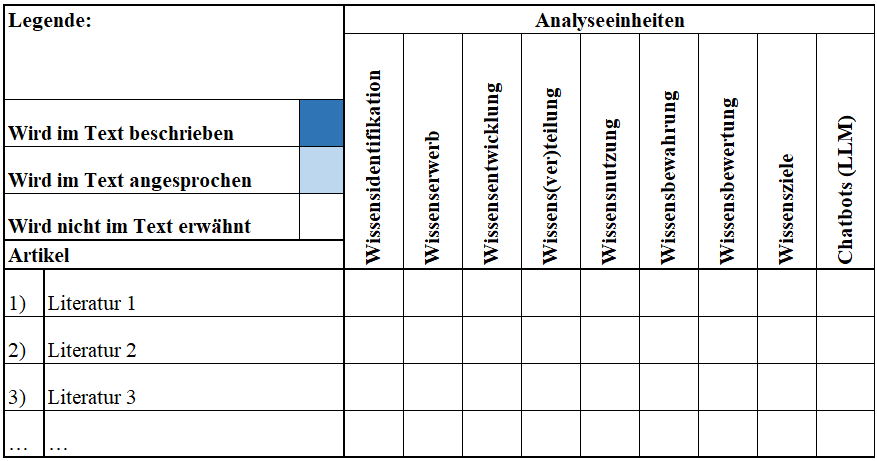
\includegraphics[width=10cm]{listings/Konzeptmatrix.png}
\end{table}


Für eine detaillierte Darstellung unseres Mondes, siehe Anhang \ref{sec:MondAnhang}.


ChatGPT-Ausgabe:
\begin{table}[h!]
\centering
\begin{tabular}{|l|l|l|l|l|l|}
\hline
1) Literatur 1 &  &  &  &  &  \\ \hline
2) Literatur 2 &  &  &  &  &  \\ \hline
3) Literatur 3 &  &  &  &  &  \\ \hline
...            &  &  &  &  &  \\ \hline
\end{tabular}
\end{table}


